\documentclass[12pt]{article}
\usepackage[a4paper, total={5.5in, 9in}]{geometry}
\usepackage{amsmath} % For mathematical formatting
\usepackage{changepage}
\usepackage[most]{tcolorbox}
\usepackage{textcomp} % for writing degrees
\usepackage{tikz} % For drawing the triangle
\usepackage{pgfplots}
\pgfplotsset{compat=1.18}
\usepackage{hyperref}

\title{Precalculus Worksheet 6.1}
\author{PCL Learning Center}
\date{}

\begin{document}
\maketitle

\begin{center}
    \textit{note: This worksheet may be used for two sessions, and\\no electronic devices may be used on this worksheet.}
\end{center}

\section*{Problem Set 1\\Difficulty level: Normal}
\subsection*{Problem 1}
Given that \(\sin(x)=-\dfrac{1}{6}\), what is \(\sin(-x)\)?

\subsection*{Problem 2}
Write the intervals where \(f(x)\) is strictly increasing on the graph of \(f(x)=\sin(x)\) in the domain \(-2\pi \leq x < 0\).

\subsection*{Problem 3}
Given that \(\cos(x)=0.37\), what is \(\cos(-x)\)?

\subsection*{Problem 4}
On the graph of \(f(x)=\cos(x)\) and the interval \([2\pi,4\pi)\), for what value(s) of \(x\) does \(f(x)\) achieve a maximum?

\subsection*{Problem 5} What is the amplitude and period of the function \(f(x)=6\sin(-3x)\)?

\subsection*{Problem 6}
What is the amplitude and period of the function \(f(x)=\dfrac{1}{6}\cos(6x)\)?

\newpage
\subsection*{Problem 7}
What is the amplitude and period for the function shown below?

    \begin{center}
    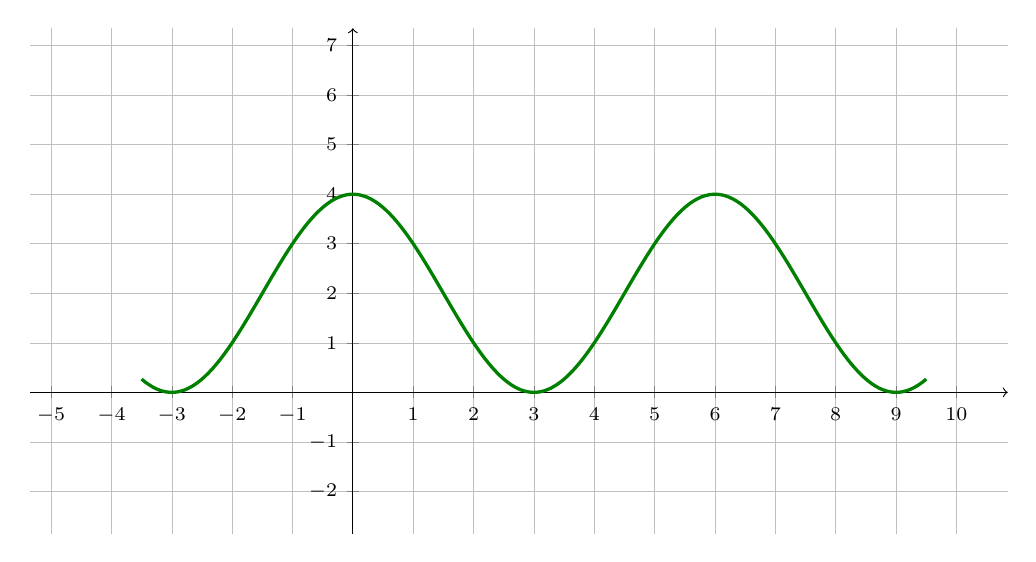
\begin{tikzpicture}
    \begin{axis}[
        width=14cm, height=8cm,
        axis lines=middle,
        ymin=-2, ymax=6.5,
        xmin=-4, xmax=9.5,
        xtick distance=1,
        ytick distance=1,
        grid=both,
        grid style={line width=.1pt, draw=gray!30},
        major grid style={line width=.2pt,draw=gray!50},
        enlargelimits=true,
        axis line style={->},
        samples=200,
        domain=-3.5:9.5,
        tick label style={font=\scriptsize}
    ]
    \addplot[very thick, green!50!black, domain=-3.5:9.5] {2*cos(deg(pi/3 * x)) + 2}
        node[pos=0.85, above] {};
    \end{axis}
    \end{tikzpicture}
    \end{center}

\subsection*{Problem 8}
Determine the magnitude and direction of the vertical shift and the phase shift for the following function.
\[f(x)=\sin\Big(x+\dfrac{\pi}{2}\Big)+2\]
The vertical shift is \underline{\hspace{1cm}} units \underline{\hspace{1cm}} (down/up), and the phase shift is \underline{\hspace{1cm}} units to the \underline{\hspace{1cm}} (left/right).

\newpage
\section*{Problem Set 2\\Difficulty level: Hard}
\subsection*{Problem 1}
Find the equation of the function show below.
    

\begin{center}
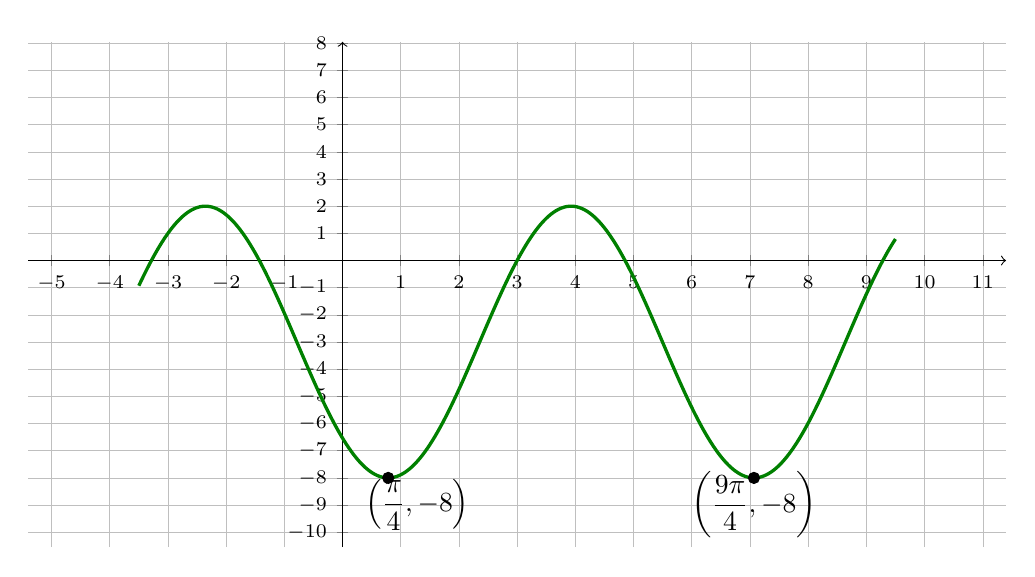
\begin{tikzpicture}
\begin{axis}[
    width=14cm, height=8cm,
    axis lines=middle,
    ymin=-9, ymax=6.5,
    xmin=-4, xmax=10,
    xtick distance=1,
    ytick distance=1,
    grid=both,
    grid style={line width=.1pt, draw=gray!30},
    major grid style={line width=.2pt, draw=gray!50},
    enlargelimits=true,
    axis line style={->},
    samples=300,
    domain=-3.5:9.5,
    tick label style={font=\scriptsize}
]

% Graficar función
\addplot[very thick, green!50!black] {5*cos(deg(x - 5*pi/4)) - 3};

% Punto mínimo en (pi/4, -8)
\addplot[only marks, mark=*] coordinates {(pi/4, -8)};
\node at (axis cs:pi/4+0.5,-9) {$\left(\dfrac{\pi}{4}, -8\right)$};

% Punto mínimo en (9pi/4, -8)
\addplot[only marks, mark=*] coordinates {(9*pi/4, -8)};
\node at (axis cs:9*pi/4,-9) {$\left(\dfrac{9\pi}{4}, -8\right)$};

\end{axis}
\end{tikzpicture}
\end{center}

\subsection*{Problem 2}
Sketch the graph of the function \(f(x)=\dfrac{1}{2}\sin(2x)+3\).

\subsection*{Problem 3}
Sketch the graph of the function \(f(x)=2\cos\Big(\dfrac{4}{3}x+\dfrac{\pi}{2}\Big)\)

\newpage
\section*{Solutions for Set 1}
\subsection*{Problem 1}
\(\sin(x)=\dfrac{1}{6}\)
\subsection*{Problem 2}
\(\Big(-2\pi,-\dfrac{3\pi}{2}\Big),\Big(-\dfrac{\pi}{2},0\Big)\)
\subsection*{Problem 3}
\(\cos(-x)=0.37\)
\subsection*{Problem 4}
\(x=2\pi\)
\subsection*{Problem 5}
The amplitude is 6 and the period is \(\dfrac{2\pi}{3}\).
\subsection*{Problem 6}
The amplitude is \(\dfrac{1}{6}\) and the period is \(\dfrac{\pi}{3}\).
\subsection*{Problem 7}
The amplitude is 2 and the period is 6.
\subsection*{Problem 8}
The vertical shift is 2 units up, and the phase shift is \(\dfrac{\pi}{2}\) units to the left.

\section*{Solutions for Set 2}
\subsection*{Problem 1}
\(5\cos\Big(x-\dfrac{5\pi}{4}\Big)-3\)
\subsection*{Problem 2}
\begin{center}
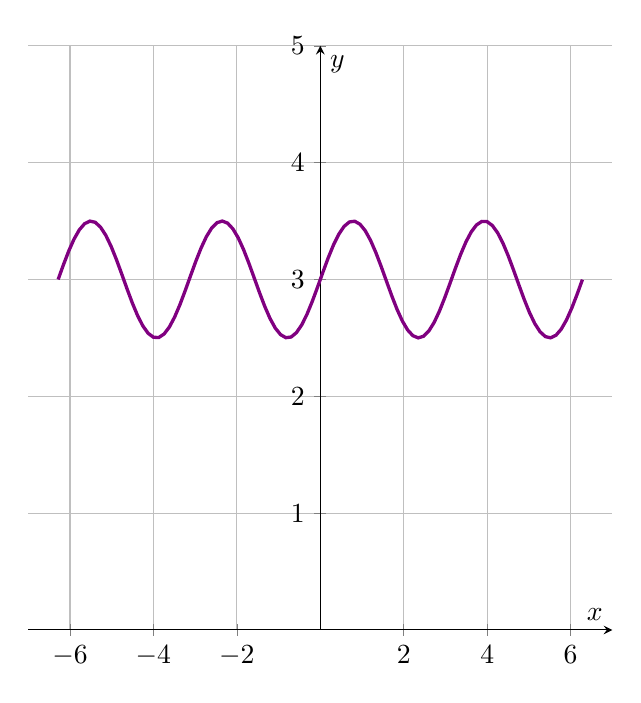
\begin{tikzpicture}
\begin{axis}[
    axis lines=middle,
    width=9cm,
    height=9cm,
    xmin=-7, xmax=7,
    ymin=0, ymax=5, 
    xtick={-6,-4,...,6},
    ytick={1,2,...,5},
    grid=both,
    xlabel=\(x\),
    ylabel=\(y\)
]
\addplot[domain=-2*pi:2*pi, samples=100, very thick, violet] {0.5*sin(deg(2*x)) + 3};\end{axis}
\end{tikzpicture}
\end{center}

For a more detailed graph, sketch \(f(x)=\dfrac{1}{2}\sin(2x)+3\) on \href{https://www.desmos.com/calculator}{Desmos} or \href{https://www.geogebra.org/graphing?lang=en}{GeoGebra} to see the solution.

\subsection*{Problem 3}
\begin{center}
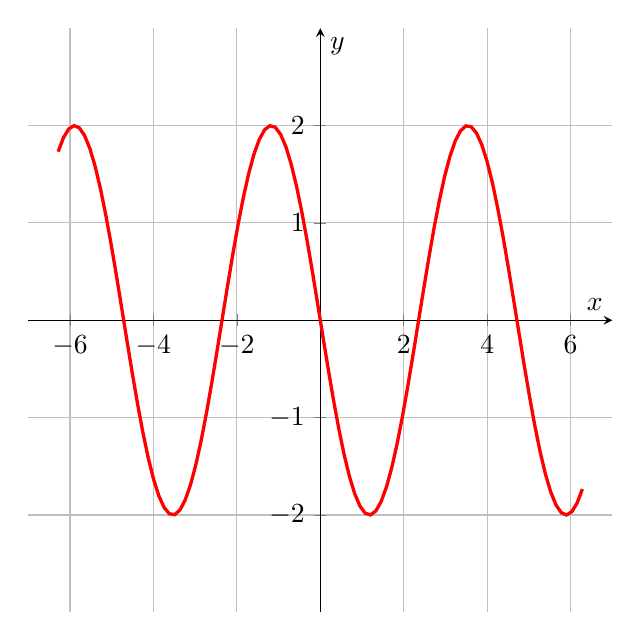
\begin{tikzpicture}
\begin{axis}[
    axis lines=middle,
    width=9cm,
    height=9cm,
    xmin=-7, xmax=7,
    ymin=-3, ymax=3, % Ajustado para la amplitud de 2
    xtick={-6,-4,...,6},
    ytick={-2,-1,0,1,2},
    grid=both,
    xlabel=\(x\),
    ylabel=\(y\),
    ]
\addplot[domain=-2*pi:2*pi, samples=100, very thick, red] {2*cos(deg((4/3)*x + pi/2))};
\end{axis}
\end{tikzpicture}
\end{center}
For a more detailed graph, sketch \(f(x)=2\cos\Big(\dfrac{4}{3}x+\dfrac{\pi}{2}\Big)\) on \href{https://www.desmos.com/calculator}{Desmos} or \href{https://www.geogebra.org/graphing?lang=en}{GeoGebra} to see the solution.

\end{document}
